\chapter{Evaluating PX in Playtherapy rehabilitation exergames}
\label{ch:playtherapy}
The goal of this project was to propose a comprehensive model to evaluate \acp{PREG} considering the entertaining and the rehabilitation purposes. In \autoref{ch:model}, we proposed a model that meets that requirement; and in \autoref{ch:methodology}, we presented a methodology to evaluate \ac{PX} in rehabilitation exergames based on that model. In this chapter, we present a study case in which we used the proposed model to evaluate \ac{PX} in a \ac{PREG}. The \ac{PREG} is called Playtherapy and is being developed by the Multimedia and Computer Vision research group from \textit{Universidad del Valle} and the Evaristo Garc\'ia University Hospital from Cali Colombia.

The remaining of this chapter is organised as follows. First, we present Playtherapy and its development environment. Then, we describe the \ac{PX} evaluation that we have conducted. Finally, we conclude the chapter presenting the main contributions and limitations of the evaluation.

To evaluate \ac{PX} in Playtherapy we employed the methodology presented in \autoref{ch:model}. \autoref{tab:conducted_evaluations} presents a summary of the evaluations conducted to evaluate Playtherapy's exergames.



\section{Antecedents}
% Game in dev
% Sessions: aspects, methods, instruments, participants
We conducted three semi-structured interviews with three physiotherapists (2 female, 1 male) from the Evaristo Garc\'ia University Hospital. We obtained informed consents from the participants verbally. The interviews were audio recorded. The goal of the interviews is to collect information about the \emph{context} where they will use Playtherapy, their expectations regarding its use and the \emph{patients' profile}. Furthermore, the game system was characterised identifying Playtherapy's architecture and using the approach presented in \autoref{sec:characterising}. Additionally, two members of the development team, a physiotherapy student and a programmer, evaluated each mini-game using the \ac{RITE} method. A summary of the evaluation process is presented in \autoref{tab:antecedents_evaluations} and detailed in the following sections.

\begin{table}[bth]
\myfloatalign
\caption{Conducted evaluation sessions to evaluate antecedents of Playtherapy}
\resizebox{\linewidth}{!}{
\begin{tabularx}{1.3\textwidth}{m{1.5cm}m{4.5cm}XXXm{1.8cm}}
%----------------------
\toprule
\spacedlowsmallcaps{Layer}
& \spacedlowsmallcaps{Goal}
& \spacedlowsmallcaps{Aspects}
& \spacedlowsmallcaps{Methods}
& \spacedlowsmallcaps{Participants}
& \spacedlowsmallcaps{Sessions} \\\midrule
Context
& Identify the profile of physiotherapists from the hospital and the hospitals' regulations required to perform an evaluation
& Rehabilitation environment
& \multirow{2}{*}{Interview}
& \multirow{2}{2cm}{3 physiotherapists}
& \multirow{2}{*}{2} \\\cline{1-3}
Player/ Patient
& Identify a general profile of patients from the hospital
& Player profile &  &  &  \\\midrule
\multirow{3}{*}{Game}
& Characterise Playtherapy's mini-games
& Characteristics
& Inspection, characterisation \autoref{sec:characterising}
& 1 \ac{PX} evaluator
& - \\\cline{2-6}
& \multirow{2}{4.5cm}{Assess whether Playtherapy meets the requirements to be used by patients}
& \multirow{2}{3cm}{Configuration capability, Tutorial quality, Movement support}
& \ac{RITE}
& 1 physiotherapy student, 1 programmer
& 10 \\\cline{4-6}
&  &  & Question asking protocol
& 1 physiotherapist, 1 physiatrist
& 5\\ \midrule
\bottomrule
\end{tabularx}}
\label{tab:antecedents_evaluations}
\end{table}

\subsection{Context}
% interviews were conducted: three participants, verbal consent, 
% Data analysed using thematic content analysis
% results: personas were developed
As described in \autoref{sec:rel_among_dimension}, the context layer comprises the cultural parameters and the rehabilitation environment associated with the use of Playtherapy. To collect data about context, we use the following guiding questions for the conducted semi-structured interviews:

\begin{enumerate}
    \item \item What activities occur during physical therapy sessions?
    \item How can a \ac{PREG} be used as part of physical therapy?
    \item How do you expect to use \ac{PREG}?
    \item How do you think \acp{PREG} should assist patients?
    \item What kind of devices and software do you use on a regular basis?
\end{enumerate}

\subsubsection{Cultural parameters}
Regarding \emph{cultural parameters}, the physiotherapists have not used \acp{PREG} in the hospital; thus, we did not identify local game communities. Some of the physiotherapists have used commercial exergames for their entertainment and outside the hospital. Only the academic community would represent an environment to share experiences and find relevant information. 

\subsubsection{Institution}
Regarding the \emph{rehabilitation environment}, the physiotherapists expressed that a typical rehabilitation therapy starts with an evaluation or diagnosis session, which will serve as input to establish rehabilitation goals and a treatment plan. A diagnosis session is performed according to the \ac{APTA} and the \ac{ICF} and may involve assessing aspects such as motion range, functional Independence, oxygen saturation, \ac{HR}, fine motor skill, balance, resistance and strength. During a rehabilitation treatment, physiotherapists perform re-evaluations periodically to assess patients progress and adapt treatment plan accordingly (e.g. by including new exercises or physical instruments). Patients' progress is tracked using forms established by the hospital. That confirms the relevance of the therapy tasks presented in \autoref{sub:def_rehab_therapy}; i.e., personalisation, supervision and assessment since they allow physiotherapists to determine whether a patient can use Playtherapy or not.

A therapy session takes one hour and comprises warm-up, cool-down and main therapeutic exercises, which are planned by a physiotherapist. In the first session, physiotherapists instruct patients to maintain a correct posture, avoid unsafe movements and take adequate precautions during exercises. Also, physiotherapists should explain and supervise each exercise execution specifying how to perform it correctly. At the end of each session, physiotherapists give feedback to patients and register important observations on a form. Moreover, auxiliary staff assist physiotherapists supervising and instructing patients. The decision to include a Playtherapy mini-game in a therapy session relies mainly on physiotherapists' criteria based on evaluation and re-evaluation results.

Playtherapy would be used in the Physical medicine and rehabilitation unit of the hospital. It has different facilities including a walk training area, a gym, a physical agents area, children area and adults area. Some of these places are usually crowded; thus, the location to use Playtherapy should be selected carefully. The unit is trying to provide two rooms to be used exclusively for playing Playtherapy.

Also, we identified internal regulations and constraints which are important to conduct an evaluation successfully. We need the approval of the head of the physical medicine and rehabilitation unit and the ethical committee of the hospital. A physiotherapist will be in charge of internal processes and logistics such as location, date, time, hospital participants and health instruments when needed. We should provide and coordinate the technical logistics.  When an evaluation requires patients' participation, we should inform the physiotherapist at least four weeks in advance to arrange an appointment; otherwise, two weeks in advance would be enough. Finally, for long-term evaluations involving patients, we need the approval of the technical committee of the physical medicine and rehabilitation unit.

\subsubsection{Physiotherapists}
About \emph{physiotherapists profile and expectations}, they expressed that they feel confident using technologies since they are used to interact with smart-phones, computers and tablets. One of them has played exergames with Kinect One and Nintendo Wii. Another physiotherapist considered herself a casual player. The physiotherapists remarked that they are in charge of deciding what a patient can do in a therapy session since they are responsible for patients' safety. The physiotherapists expect Playtherapy to add variety and dynamism to the therapies they conduct, aid patients to reach the rehabilitation goals, motivate patients to perform the expected rehabilitation movements while reaching game goals, provide patients with information about goals, performance and progress. Moreover, they require Playtherapy to be an assisting tool that can be configurable to patients' needs and preferences (to assure patients' safety) and offer the possibility to work on particular joints and movements. They do not want Playtherapy to increase their workload. \autoref{fig:physio_personas} presents the two persona models that we built based on collected information.

\begin{figure}[bth]
\centering
 \subfloat[Physiotherapist with average IT mastery]{
   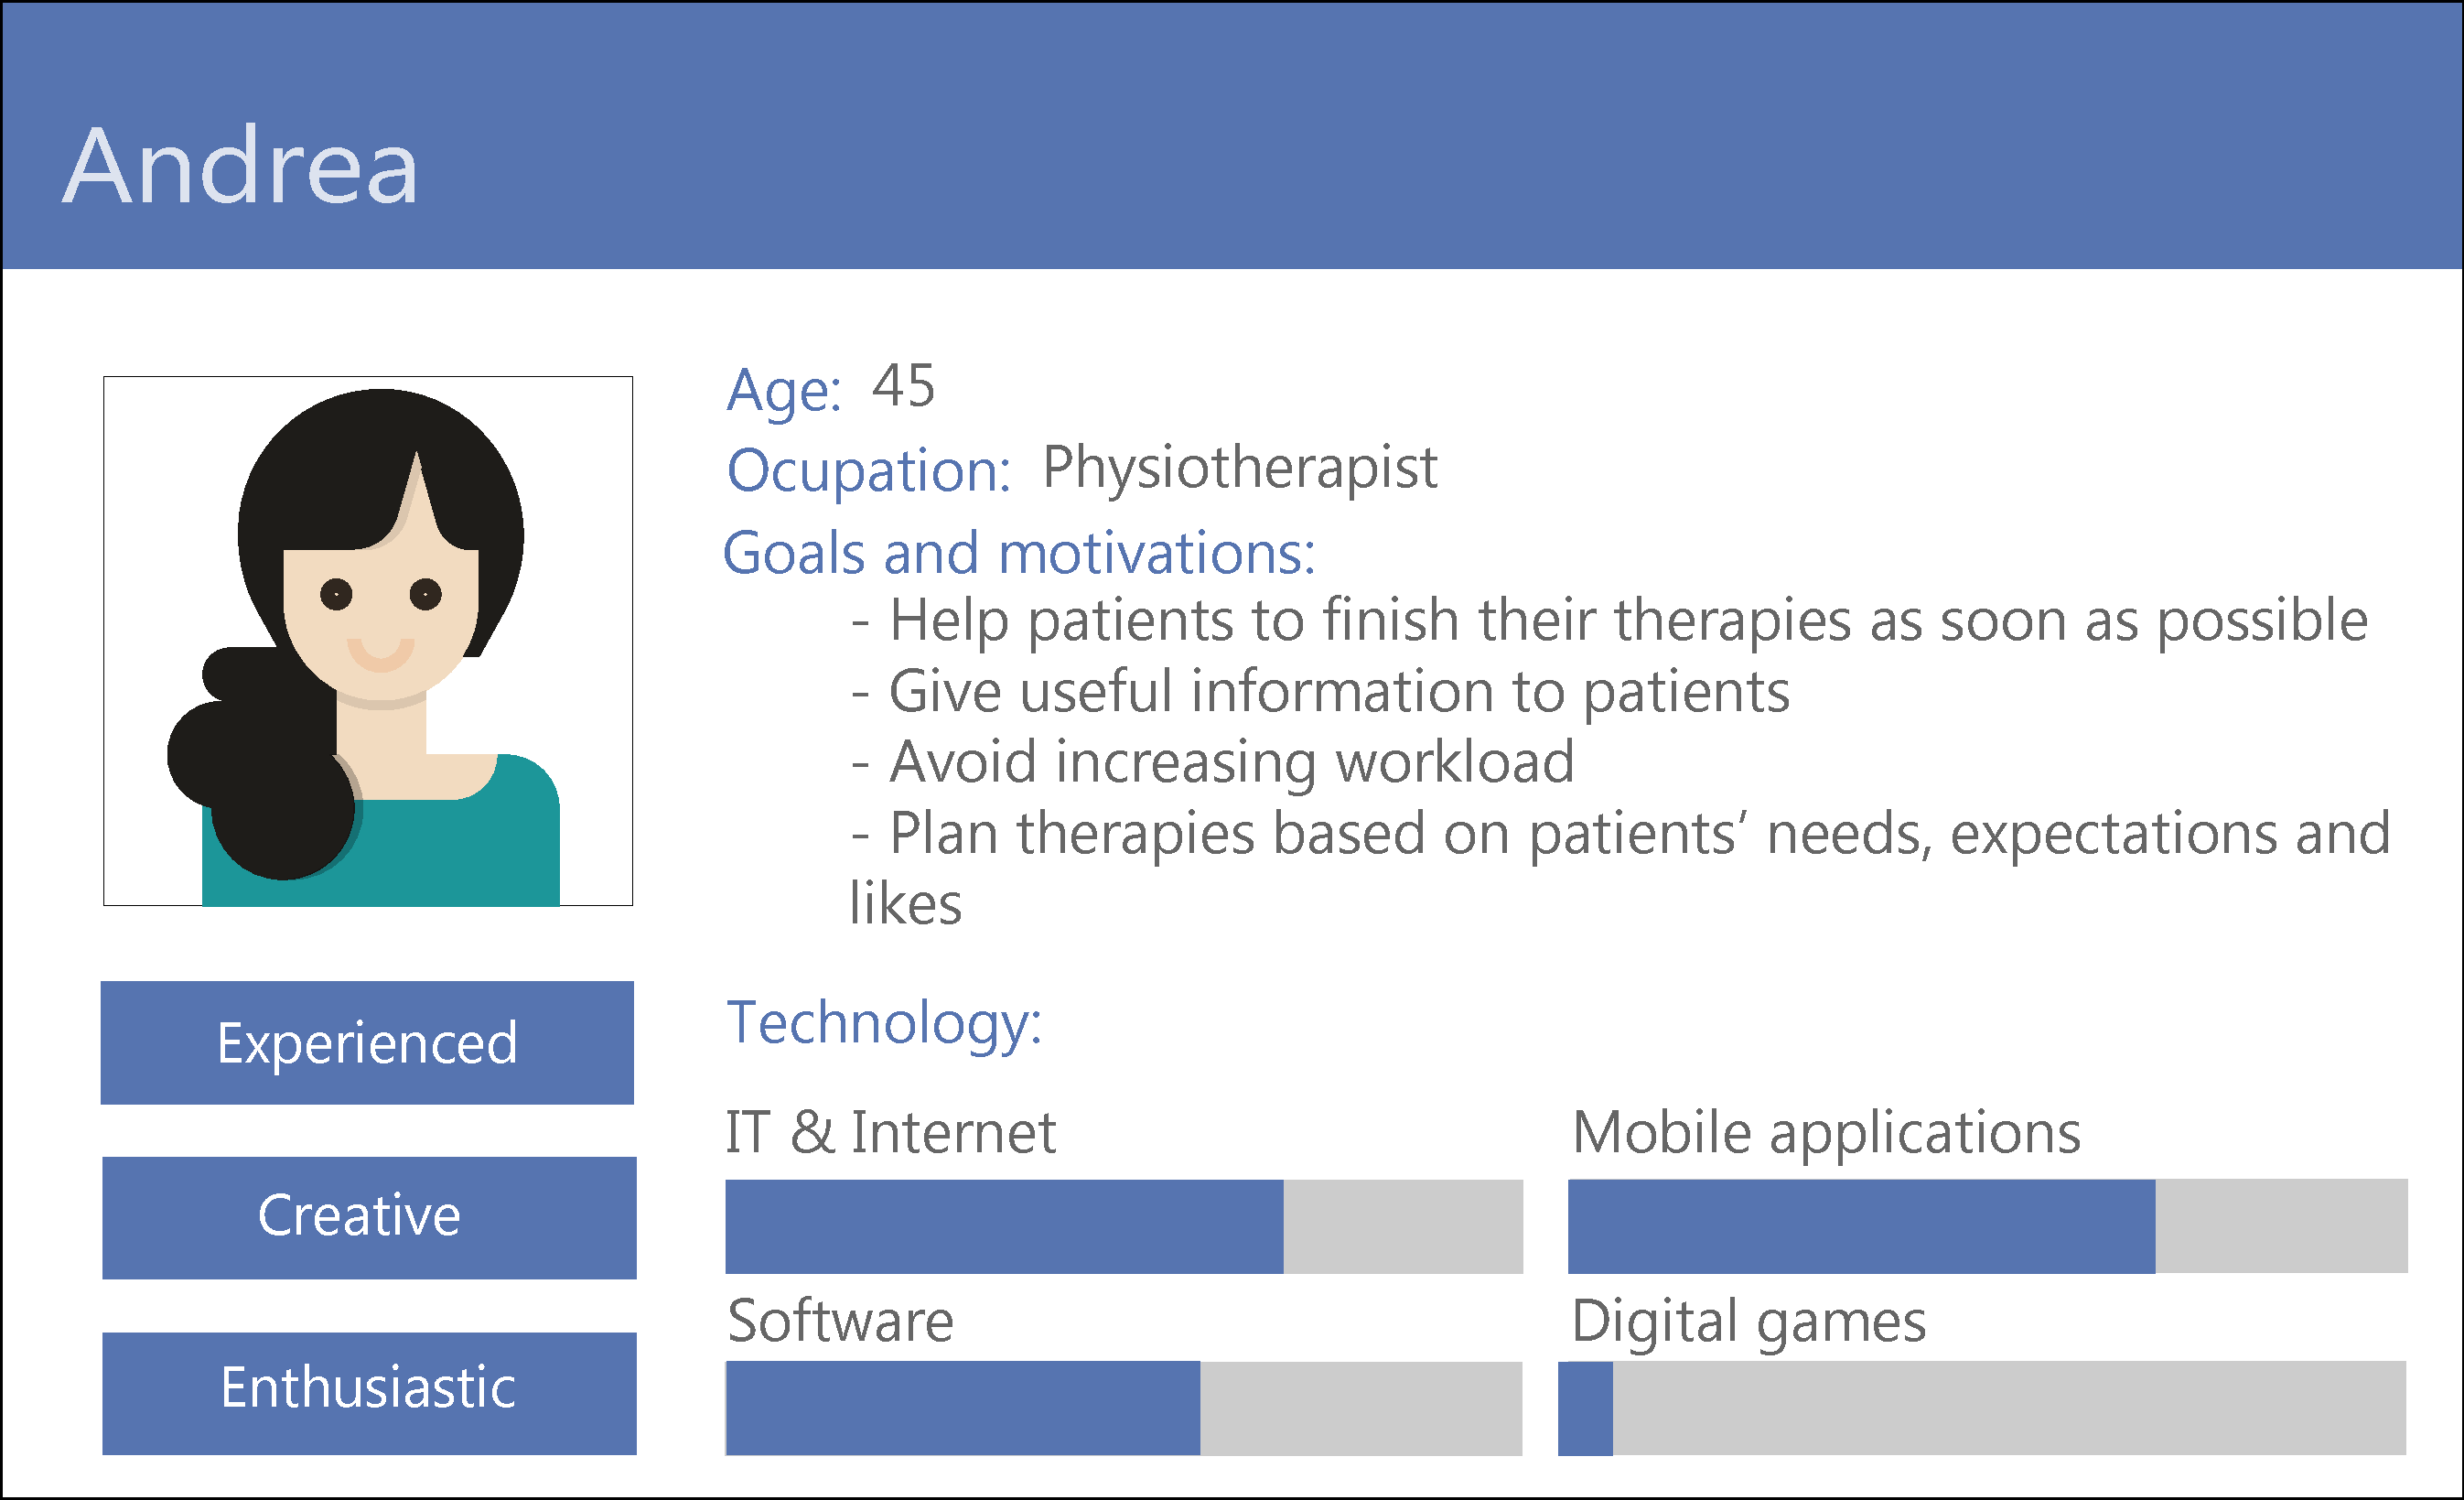
\includegraphics[width=0.48\linewidth, frame]{gfx/playtherapy/personaPhyAndrea}
   \label{fig:personaPhyAndrea}
 }
 \subfloat[Physiotherapist who sympathises with games]{
   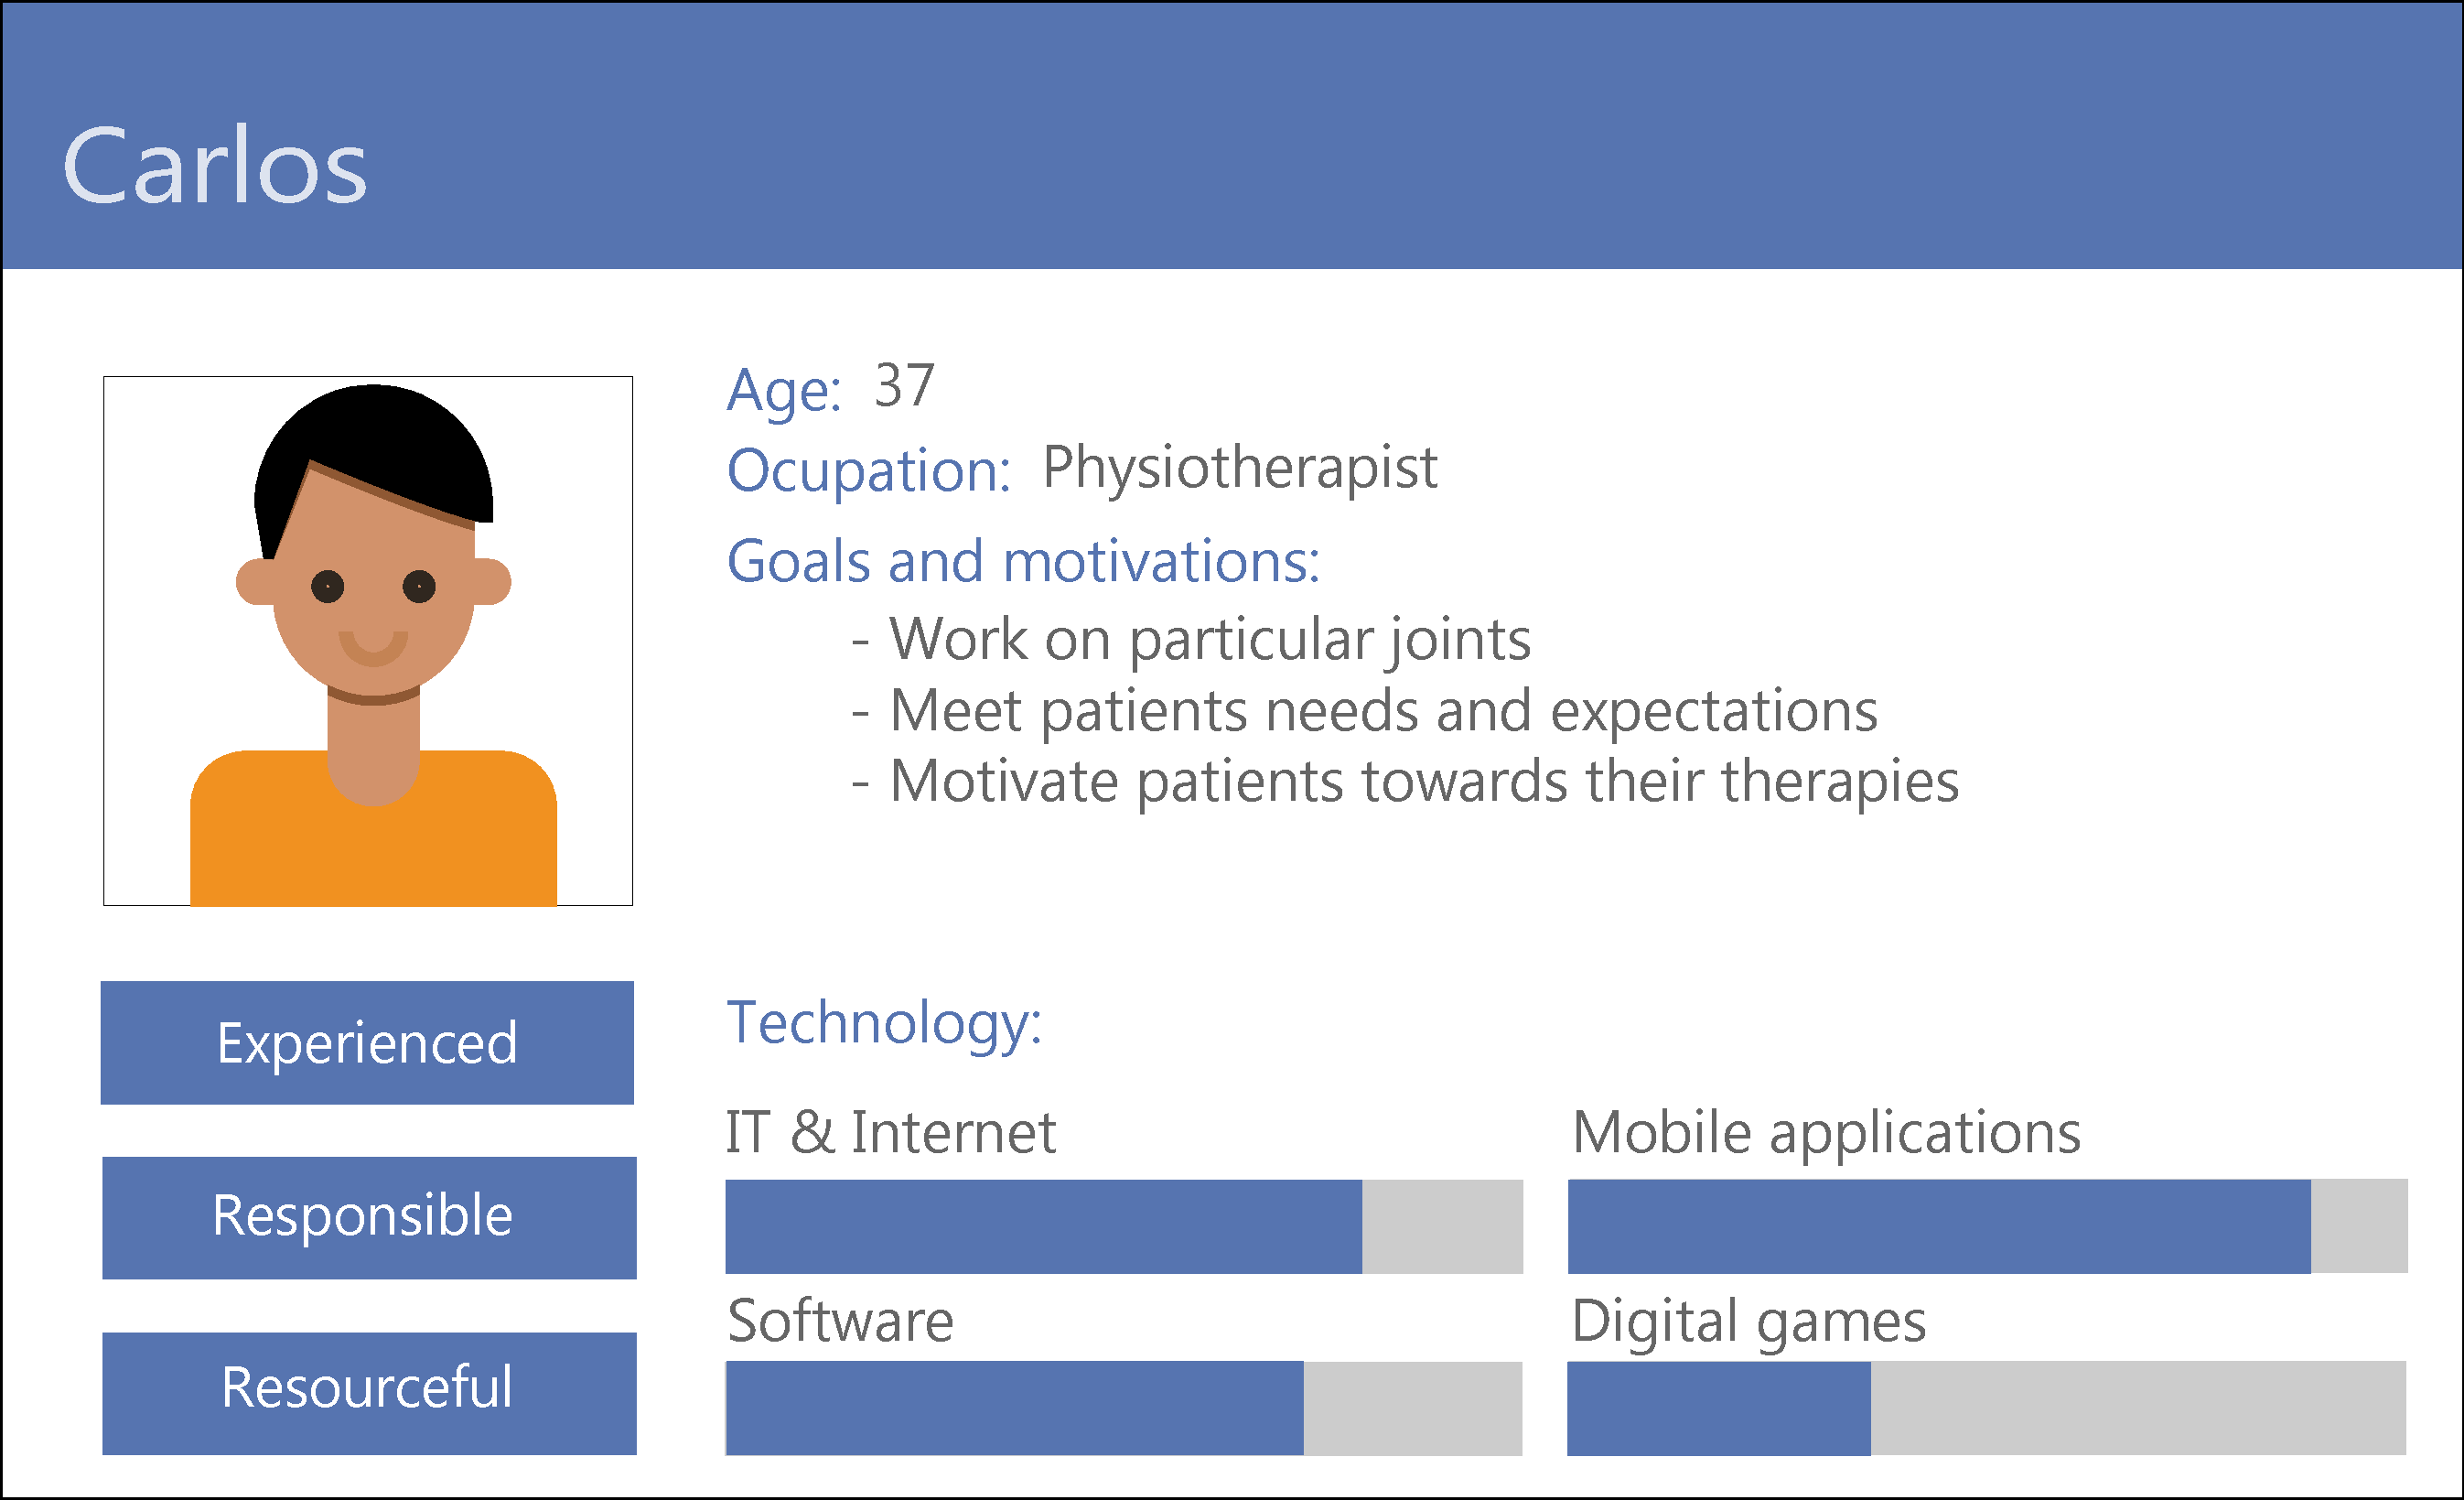
\includegraphics[width=0.48\linewidth, frame]{gfx/playtherapy/personaPhyCarlos}
   \label{fig:personaPhyCarlos}
}
\caption{Physiotherapists' persona models}
\label{fig:physio_personas}
\end{figure}

\subsection{Player/Patient}
Following the proposed model \autoref{sec:rel_among_dimension}, we identified characteristics, motivations and expectations of patients of the hospital to build Persona models. We use the following guiding questions to collect the data:

\begin{enumerate}
    \item What kind of patients participate in physical therapy?
    \item How is patients' motivation towards physical therapy?
    \item What factors affect patients' motivation towards physical therapy?
\end{enumerate}


Specific information about game activity, health status and previous experiences of players is collected before conducting any evaluation of \emph{Interaction} that involves patients (See \autoref{sec:interaction_eval}).

\subsubsection{Demographic characteristics}
The physiotherapists expressed that patients who require physical therapies have musculoskeletal, cardiopulmonary and neuromuscular pathologies including lower and upper limbs fracture or traumas, cerebral palsy, joint dislocation and stroke. In the case of Playtherapy, it would be targeted at musculoskeletal patients since they require active exercises. Chronic patients are those who have a very limited range of motion of one or more joints.

Regarding age, the physical medicine and rehabilitation unit of the hospital treats children from five to twelve years old. However, most patients are over the age of eleven. Also, young patients (thirteen to seventeen years old), young adult patients (seventeen to thirty-five years old), adults (thirty-six to sixty years old) and elderly patients (older than sixty years old) are treated.

Most children who are treated at the unit are attending primary school. Most young patients have finished primary school and attend secondary school, though, some of them quit before finishing it since they start working. Most young adults have finished secondary school or are finishing it. Some of them have completed a technical career. Most adult and elderly patients have finished at most primary school. Few of the adults have finished secondary school.

Most children who are treated at the unit are attending primary school. Most young patients have finished primary school and attend secondary school, though, some of them quit before finishing it since they start working. Most young adults have finished secondary school or are finishing it. Some of them have completed a technical career. Most adult and elderly patients have at most finished primary school. Few of the adults have finished secondary school.

The unit treats female and male children proportionally. Young and young adult patients are mainly male. Meanwhile, adult and elderly patients are mostly female. All patients belong to the lower or working classes; i.e., one, two and three Colombian social strata.

Regarding the work with patients, the physiotherapists commented that children and young patients are willing to work during the therapy sessions and understand what they should do easily. Young adults and adults do not like reading and prefer visual aids. Finally, physiotherapists should monitor elderly patients closely since they have comprehension difficulties and get confused with the instructions easily.

\subsubsection{Motivations and expectations}

% Las mayor expectativa del paciente es finalizar la terapia rápido

% Los pacientes se demotivan por la repetición y monotonía de los ejercicios
% El paciente quiere saber cuánto dura su tratamiento de recuperación

%Si tiene una razón externa, ej: trabajar, poder reintegrarse a la vidad diaria: vestirse, peinarse, ...; para lograr el objetivo terapeutico, entonces puede estar motivado

% Si el pacietne es juciosos y continúa los ejercicios en casa puede tener mejor progreso -> motivación

% Adultos tempranos y mayores, son más grupales que individuales. Clase de pilates, clase de yoga, usar un deporte inclusivo

% Con los niños se trabaja con juegos
% El ínteres de los pacientes es una recuperación pronta
% Los niños debe ser más interactivos, dinámicos. Con juego
% Niños juegos, ayudas didácitca, visual
%Disposición en niños es alta. Con ellos es díficl lograr atención. El mismo ejercicio los aburre. Se debe ser recursivo, quieren hacer muchas cosas. 

% Jóvenes, coversar sobre temas de ínteres, usando ayudas didacticas ayuda a motivarlos
% Jóvenes son dispuestos, se prestan muchoa las recomendaciones hechas por los fisioterapeutas
% Disposición en jóvenes, adultos temprano y medio dispuesto colaboradores.

% Disposición mayores: la edad es una limitación, puede ser díficil realizar un ejercicio
% Disposición mayores: la edad es una limitación, puede ser díficil realizar un ejercicio

% Los pacientes pueden mejorar su disposición si el fisioterapeuta agrega variedad a la terapia, ej: incrementando dificultad. inluyendo nuevos elementos. Depende de la creatividad del fisio

\subsection{Game system}

\subsubsection{General characteristics}
Playtherapy is a collection of mini \acp{PREG} whose purpose is to increase patients' motivation towards completing their physical rehabilitation therapies. Playtherapy is being developed by the Multimedia and Computer Vision research group from \textit{Universidad del Valle} in collaboration with the Physical Medicine and Rehabilitation Unit of the Evaristo Garc\'ia University Hospital from Cali Colombia.  

Playtherapy's \acp{PREG} are designed to assist patients to recover motion of particular joints, thereby being oriented to movements rather than pathologies. It is a generic tool that may be used with patients having different pathologies. As a consequence, two key elements of Playtherapy are the number of mini-games it contains and the coverage of joints it supports.

Playtherapy is being developed following an iterative and incremental methodology, which is appropriate for game development. The methodology is called Game-Scrum and consists in developing digital games using SCRUM agile practices along three stages: pre-production, production and post-production \autocite{godoy2010game}.

During \emph{pre-production} developers define an initial and general idea for the game, it comprises, among other aspects, its characteristics, rules, controls, art and sound. Developers perform activities such as brainstorming, prototype development, game sessions and technologies exploration are performed. The outcome of this stage is a \ac{GDD}. Then, in \emph{production} stage, developers define the game's \textit{product backlog} using the \ac{GDD} of the previous stage as input. This phase progresses following the roles, artefacts and meetings of SCRUM \autocite{keith_agile_2010}. Finally, \emph{post-production} includes evaluating the game being developed and the creation of a \textit{postmortem} to collect learned lessons that can be used in future projects.

Each \ac{PREG}, including its thematic, main objectives, rules and mechanics were designed during weekly brainstorming sessions involving the participation of a physical therapy undergraduate student. Additionally, regular meetings with a group of physiotherapists from a local hospital were arranged, where continuous feedback was received to develop, validate and improve every implemented feature; so that the exergames could meet both physiotherapists' and patients' needs.

Playtherapy is developed in an academic environment. The defined sprint length for the project is two weeks. As expected, a sprint planning, a sprint review and a retrospective meeting are performed every sprint. The development team is composed as follows:
\begin{itemize}
    \item \emph{System engineering undergraduate students}: they are responsible for the video game implementation; i.e., they develop every user story related to the project. Also, they are responsible for performing functional testing and adapt Playtherapy according to the results obtained after user acceptance tests and \ac{PX} evaluations performed with physiotherapists and patients. In the context of SCRUM methodology, those students play the role of development team members.
    \item \emph{Physiotherapy undergraduate student}: she is responsible for guiding the previous team in aspects related to the physical rehabilitation field. Further, she approves acceptance tests and participates in the validation of the employed technologies and exergames. According to SCRUM, that student plays the role of a development team member.
    \item \emph{Systems engineering master student}: he is responsible for leading the development process, coordinating every meeting and practice proposed by the SCRUM methodology. He plays the role of a SCRUM master role.
    \item \emph{Physiotherapist}: a physiotherapist participates in every sprint review meeting to validate all implemented features and guarantee that the exergame meets the patients' needs. His/her role is \textit{product owner} according to SCRUM methodology.
\end{itemize}

All team members participate in generating ideas to design and implement every mini \ac{PREG}. The goal of having an interdisciplinary team is to explore different possibilities and validate their viability regarding physical rehabilitation needs and technology capabilities.

\subsubsection{Characteristics of the mini \acp{PREG}}
Playtherapy covers a set of rehabilitation movements and exercises using mini \acp{PREG} that support specific joint movements. Each mini \ac{PREG} is designed to be personalised by physiotherapists to adapt to patients' needs and offer a compelling and natural experience. An exergame comprises a set of components, which were created to assist physiotherapists work and enhance patients' experience when interacting with a mini-game. These components are illustrated in \autoref{fig:mg_arch}.

The \emph{GUI} component is composed of the screens that each exergame has. Each screen was created following a standardised design pattern and usability guidelines related to colour and elements distribution. There are three main screens. First, the  \emph{parameters screen} which allows physiotherapists to set up a mini \ac{PREG} before it starts to adapt the game session to patients' particular needs (See \autoref{fig:parameters_screen}). A mini \ac{PREG} is configurable through a set of parameters, such as movement angle thresholds, choosing between repetition based or session time-based session and enabling or disabling joints and exercises. Every parameter configuration was agreed on with the physiotherapists who supported the development process. Second, the \emph{tutorial screen} explains the game objectives, rules and mechanics (See \autoref{fig:tutorial_screen}). Additionally, the tutorial includes visual representations of the movements that a player/patient has to perform, which allows therapists and patients to understand how to play and interact with the game. Finally, the \emph{results screen} shows the performance obtained by a player/patient along with visual feedback after a game session (See \autoref{fig:results_screen}). The visual feedback is always positive since Playtherapy is a game intended to motivate and distract players/patients from their environment. Therefore, players/patients always receive a reward disregarding how well they perform.
    
The \emph{world} component comprises the elements related to the exergame environment. These elements are mainly 3D models and materials that make up the background objects and interaction elements of the exergame (See \autoref{fig:world_screen}). This world comprises the elements. First, the \emph{game scenario} includes all the background elements that constitute the world of the game, such as terrains, background nature and buildings, skyboxes, and any other non-interactive game objects. Second, the \emph{interaction elements} comprise specific objects that players interact with by performing different movements and exercises associated with the \ac{PREG}. Third, \emph{feedback effects} are triggered to help players/patients be conscious of the outcomes of their actions. Fourth, the \emph{final animation} indicates players/patients that a mini-game session has ended. The goal of this component is to provide a smooth and compelling transition from the game end and the Results Screen. This transition was denominated the Final Animation and consists in a sequence of game objects behaviours that dynamically and graphically illustrate the end of a game session.

The elements of the \emph{logic} component are mainly scripts that define the different rules, mechanics and behaviours of the exergames. Logic is structured as follows a \emph{game manager} controls \ac{PREG}'s flow and state. It determines and controls when the game starts, pauses and ends. It also keeps track of the current score of a player, updating it according to each player movement. It controls exergame behaviour according to configured parameters signalling corresponding events and actions. A \emph{movement control} component communicates with tracking devices' APIs to get the required data, such as joint position and rotation. Then, it performs corresponding calculations to determine if a player has performed a certain movement or exercise. A \emph{persistence} component stores patients' performance based on the obtained score and range of motion progression. This information is used by a web application, that belongs to Playtherapy, to generate reports.

\begin{figure}[h]
\centering
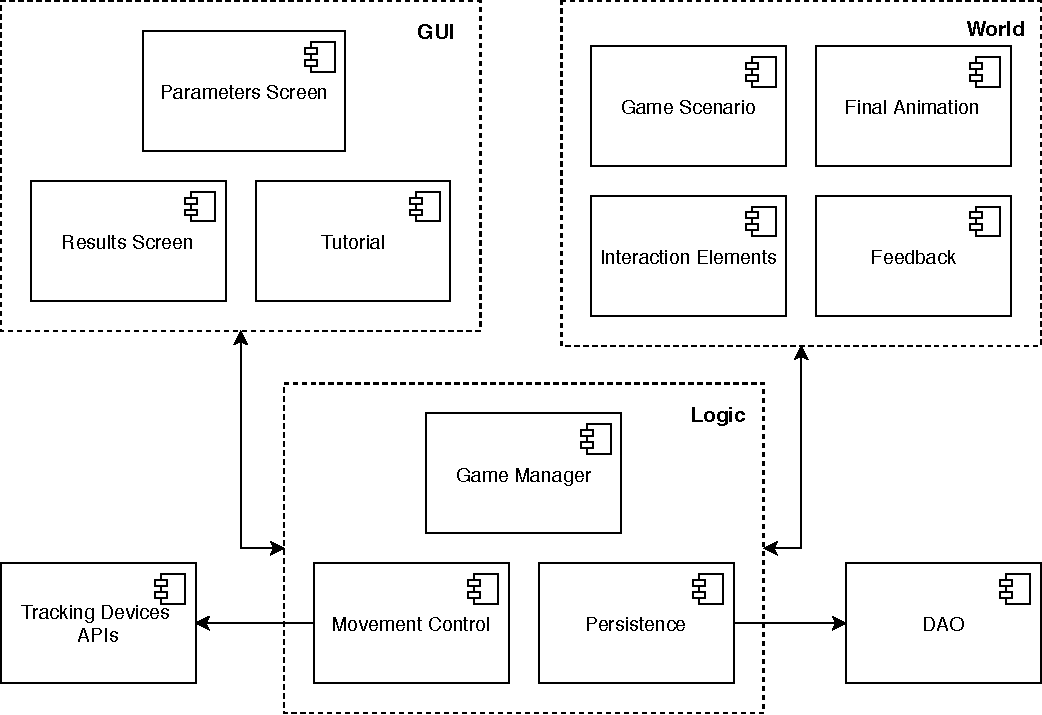
\includegraphics[width=.9\linewidth]{gfx/playtherapy/minigame_architecture}
\caption{Playtherapy's exergames architecture}
\label{fig:mg_arch}
\end{figure}

\begin{figure}[bth]
\centering
\subfloat[\textit{Piano}'s parameters screen]{
   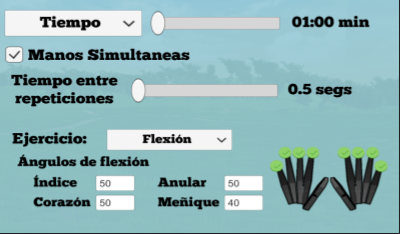
\includegraphics[width=0.4\linewidth, frame]{gfx/playtherapy/parameters_screen}
   \label{fig:parameters_screen}
}
\subfloat[\textit{Rieles}' tutorial screen]{
   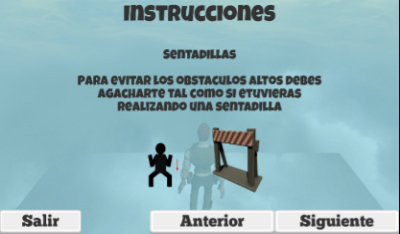
\includegraphics[width=0.4\linewidth, frame]{gfx/playtherapy/tutorial_screen}
   \label{fig:tutorial_screen}
}\\
\subfloat[\textit{Tiro Libre}'s results screen]{
   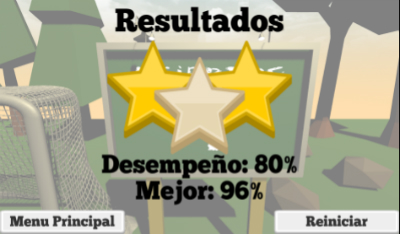
\includegraphics[width=0.4\linewidth, frame]{gfx/playtherapy/results_screen}
   \label{fig:results_screen}
 }
 \subfloat[\textit{Tiro Libre}'s game world screen]{
   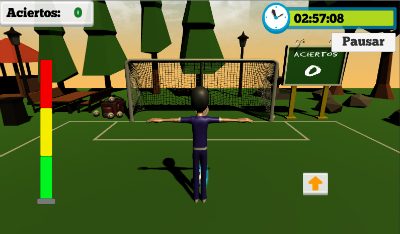
\includegraphics[width=0.4\linewidth, frame]{gfx/playtherapy/world_screen}
   \label{fig:world_screen}
}
\caption{Playtherapy's \acp{PREG} main screens}
\label{fig:platherapy_screens}
\end{figure}

Playtherapy is composed of fifteen mini-games which are briefly described below. Moreover, a characterisation of one the mini \acp{PREG} is presented in \autoref{tab:beisbol_char}, it uses the approach presented in \autoref{sec:characterising}. The characterisation for all mini \acp{PREG} is available online\footnote{\url{https://docs.google.com/spreadsheets/d/1b7AP9cNvmY6BVOT0HFJV8h7jyw7y8L7hEqteZ-woMQ0/edit\#gid=0}}.

\begin{enumerate}
    \item \emph{Tiro Libre}: players perform kick movements to strike a ball against some targets placed in a goal. It should support right/left hip flexion and extension and lateral shifts.
    \item \emph{Rieles}: players jog to go forward and squat and jump to avoid obstacles while collecting coins. It should support jumps, squats, jogging and lateral shifts.
    \item \emph{El Gran Viaje}: players control a plane moving their body to collect gems and avoid obstacles. It should support right/left hip abduction, lateral and frontal trunk inclination and squats.
    \item \emph{Estilo Libre}: players have to maintain a ball in the air using their legs. It should support right/left hip flexion and extension.
    \item \emph{Sushi Samurai}: players cut fishes coming out of the water. It should support right/left shoulder and elbow flexion and extension.
    \emph{B\'eisbol}: players have to grab balls being thrown at them using their arms. It should support right/left shoulder abduction or extension, elbow flexion and extension.
    \item \emph{Fight}: players use their arms to perform magic tricks and defend the city. It should support right/left shoulder and elbow flexion and extension.
    \item \emph{Figuras M\'agicas}: players have to draw figures using their hands to eliminate approaching enemies. It should assist in hand-eye coordination.
    \item \emph{Piano}: players have to perform finger movements to play a piano keyboard. It should support fingers flexion, extension and oppositions.
    \item \emph{Topos}: players perform grabbing movements (fist) to catch moles or directly touch them by moving their hands. It should support hand touch and grab.
    \item \emph{Vecinos Invasores}: players have to defend farm animals from being abducted by destroying alien ships using their hands. It should support hand touch and fingers oppositions.
    \item \emph{Viajando en el Espacio}: players control a spaceship using their hands to collect stars and overcome obstacles. It should support ulnar and radial deviation, wrist flexion and extension and hand grab.
    \item \emph{Dulce Hogar}: players control a cat using their hands to collect stars and avoid enemies. It should support ulnar and radial deviation, wrist flexion and extension.
    \item \emph{Cavano}: players control a bowl using their hands to gather falling objects and drop them into a jar. It should support pronation and supination.
    \item \emph{Guerra Medieval}: players have to defeat enemies using hand movements. It should support ulnar and radial deviation, wrist flexion and extension and hand grab.
\end{enumerate}

\begin{table}[bth]
\myfloatalign
\resizebox{\linewidth}{!}{
\begin{tabularx}{1.2\textwidth}{p{5cm}X}
%----------------------
\toprule
\spacedlowsmallcaps{Property}
&\spacedlowsmallcaps{Value}\\\midrule
Rehabilitation type & Tight-focused \\\midrule
Assisted Tasks & Configuration, personalisation and motivation \\\midrule
Degree of autonomy & Second degree \\\midrule
Configuration and assessment & Close-loop (Online motion range measurement)\\\midrule
Input interaction device & Camera tracking: Kinect 2\\\midrule
Output interaction device & Traditional: TV screen, speakers\\\midrule
Thematic content & Imaginary\\\midrule
Type of intervention & Individual \\\midrule
Location & Physical medicine and rehabilitation unit of Evaristo Garc\'ia University Hospital\\\midrule
Movements & Right/left shoulder abduction and/or extension, elbow flexion and extension\\\midrule
Configuration parameters & Game mode, left/right shoulder selection, minimum angle and maximum angle per movement, radius (reformulated as Movement action radius), ball speed\\\midrule
Rehabilitation goal(s) & Patient increases shoulder abduction or extension range of motion\\\midrule
Health instruments & Goniometer\\\midrule
\bottomrule
\end{tabularx}}
\caption{Characterisation of \textit{B\'eisbol} mini \ac{PREG}}
\label{tab:beisbol_char}
\end{table}

Furthermore, Playtherapy has an accompanying web application composed of three main modules. The first module is concerned with patients and physiotherapists demographic data. The second module allows physiotherapists managing patients \ac{FIM}. Finally, the third module allows visualising mini-game sessions data; e.g., registered observations, progress over time and performance measurements, like the maximum range degree achieved per session. By the time this master project took place, this application was still under development and was not connected to Playtherapy \acp{PREG}; thus, it was not evaluated.

\subsubsection{Rehabilitation support}
As described in \autoref{sec:characterising} the rehabilitation support aspect comprises assessing movement support and configuration and personalisation capability. The goal of evaluating rehabilitation support is to assure that the evaluated \ac{PREG} can be used to assure patients' safety. Therefore, we performed an \emph{internal evaluation} with two members of the development team, a physiotherapy student and a programmer, who conducted ten sessions of \ac{RITE} testing.

The physiotherapy student tested all Playtherapy's \acp{PREG}. To assess \textit{configuration capability}, she tested each configuration parameter to assess whether it behaved as expected and was easy to understand. Moreover, she tested whether the expected \textit{movements were correctly mapped} and detected by each mini \ac{PREG}. Additionally, she evaluated the \textit{quality of the tutorials} assessing the content and the coverage of the associated movements regarding the game mechanics. When she identified an error or an enhancement, the programmer fixed it and the student test it again until it was correct.

The results of the \ac{RITE} evaluation were mainly improvements related to the phrasing of configuration parameters and tutorial instructions. The student assessed their clarity from the physiotherapists' and patients' point of view. Similarly, she suggested to include graphics or animations to make the instructions and movements clearer. She configured the games considering different (ad-hoc) scenarios, exploring different game modes, including and excluding movements and modifying their difficulty. While testing each scenario, she also assessed the visibility of game objects and relevance of the visual and auditory feedback related to the game goals, leading to the inclusion of visual animations and sounds (e.g., to indicate the corresponding joint to execute a certain movement).

After the internal evaluation, we conducted five evaluation sessions of one hour using the question asking protocol and involving one physiotherapist and on physiatrist of the hospital. The purpose of this evaluation stage was to validate the results of the evaluation conducted with the development team. Eight mini \acp{PREG} were tested in this evaluation; i.e., \textit{Béisbol, Fight, Tiro Libre, Guerra Medieval, Estilo Libre, Figuras Mágicas, Gran Viaje} and \textit{Vecinos Invasores}. The last eight of these mini \acp{PREG} had been tested by the physiotherapist; thus, fewer issues were identified for those.

The participants were asked to configure at least two game sessions for each mini \ac{PREG}. After configuring one game session, they played it to identify errors or improvements. The first configuration was suggested by the evaluator, and the others were proposed by the participants. During the whole process, they could express their thoughts and impressions loudly . The evaluator could ask questions when needed. We took notes of the findings during the evaluation.

Initially, \textit{Béisbol} mini \ac{PREG} had a name in English (Baseball); however, the participants suggested to use the same name in Spanish due to the low level of patients' literacy. They expressed that understanding the game name was important to understand the game. Also, they remarked that game should indicate the patients where they should position the avatar before starting the game; they suggested to include a position mark and ask patients to move towards it. Moreover, they requested to rename one of the configuration parameters from \textit{Ratio} to \textit{Action ratio} (in Spanish) for understanding purposes. This parameter indicates the distance between the thrown ball and the patients' hands, depending on its value patients should stretch their arms or perform elbow flexion and extension movements. They suggested some rephrasing for the tutorial instructions. Regarding, movement mapping correctness, all movements were mapped correctly. However, they detected that a reduced shoulder abduction could be detected as shoulder extension. Finally, they suggested to include a visual mark indicating the position where patients should catch the balls to foster correct movement executions.

Similarly, the participants suggested to rename \textit{ABC} since its original name was in English (Fight). Also, the game displayed some visual objects to determine whether the patient should perform elbow movements. However, this was not explained in the tutorial. Thus, they requested to include that information.

About \textit{Tiro Libre}' parameters screen, the participants requested to use the term coronal plane instead of frontal plane for one of the parameters. Also, they suggested to group the \textit{Lateral shifts} and \textit{Frequency} parameters visually since they are related. Additionally, they noticed that a bar that represented the final height of a kicked ball was placed horizontally and suggested position it vertically. In the tutorial, they suggested changing the figures to differentiate lateral from frontal movements. Also, the dynamic help offered by the game was not explained in the tutorial.

Regarding \textit{Guerra Medieval}, the participants suggested to visually separate two excluding parameters. Also, the screen allowed to include pronation and supination movements, however, the game mechanics do no use them. Thus, they requested to remove them. Although the players control a virtual cannon in the game, they suggested to include virtual hands to help players be conscious of the movements they are performing. Also, they identified some typos in the tutorial and suggested to include more graphical aids and reduce the amount of text.

They detected that the performance measure presented by \textit{Estilo Libre} at the of a game session was calculated incorrectly. About the tutorial, they noticed that there was no back button to read previous instructions. Moreover, they requested some rephrasing and to modify the images to differentiate lateral from frontal movements. Regarding the parameters screen, they detected that changing the value of the \textit{Dynamic help} parameter caused no effects since the dynamic help was always presented.

About \textit{Figuras Mágicas}, the participants made some suggestions about the phrasing of the tutorial instructions. Moreover, when playing by repetitions in \textit{Gran Viaje}, the participants detected that the game requested players to execute more movements than expected. Meanwhile, they suggested some rephrasing to the tutorial of \textit{Vecinos Invasores}, and requested to remove the \textit{Pinch force} parameter since force cannot be measured by the game.

\section{Interaction}
\label{sec:interaction_eval}

\section{Effects}

\section{Discussion}
After summarising the results of the conducted evaluations, the following results were obtained:

One of the key features of Playtherapy is the configuration parameters screen, available for each mini-game, which allows personalising therapy sessions by setting exergames parameters according to the needs of a patient. The feedback received from the physiotherapists was in general positive, they expressed that it was quite helpful to be able to configure a mini-game for different patients and pathologist, and the screen was easily manageable and understandable. In the evaluations with the physiatrist and the physiotherapists all the parameters were correct since the exergames behave as expected. Their recommendations were about renaming parameters, rephrasing some tutorial instructions or adding graphical explanations to the tutorials. Only one game exergame (B\'eisbol) presented an issue regarding a movement that was not correctly mapped. Those results may be because the physiotherapy student inspected each exergame during six months and all of her recommendations were attended as soon as the appeared.

Regarding patients the evaluations that involved patients. They described both exergames as a dynamic alternative to the therapy routine. They felt immersed in both exergames since they got not distracted from the rehabilitation environment. Patients expressed their motivation and eagerness to keep playing and were enthusiastic at the fact that they could play a game while completing their rehabilitation treatments. We received some recommendations about colour combinations to improve the contrast of objects, improving their visibility to patients.

Physiotherapists described Playtherapy as an assistant tool in physical rehabilitation therapies, because it represents a dynamic alternative to therapy routine, allowing patients to have fun and also being distracted from their environment. Additionally, the physiotherapists mentioned that more exergames would be helpful, including other movements to support other exercises, as more movements may provide more flexibility during therapies.

The exergames include objectives and challenges that provide rewards when completed, motivating patients to perform better at a game and also perform the exercises needed to achieve a certain goal. Moreover, every exergame provides positive feedback when performing well, and encouraging feedback when not so well. Thus, patients may feel motivated to perform therapy sessions if they know they are also going to perform an activity they like.

According to physiotherapists feedback, Playtherapy is a promising rehabilitation tool based on configuration, personalisation, and assessment. Some reasons may be: (i) each mini-game design process was driven by rehabilitation exercises, (ii) each mini-game has an associated screen parameter to allow offering a personalised session for patients, and (iii) data collected during therapy game sessions can be managed and visualised using the web application.

The obtained positive results may be a consequence of using an incremental and iterative methodology involving physiotherapy experts along the whole development process. Expert participation allowed to understand real patients and physiotherapists' needs and expectations. Consequently, an enhanced version of each exergame was developed after each evaluation, considering feedback, proposals and suggestions received from both the physiotherapy student and the physiotherapists. 

Additional evaluations of patients' motivation and engagement may be performed since current results may be due to the novelty of the employed devices. The evaluation that we have conducted allowed us to assess the antecedents and in some degree the interaction moment of \ac{PX} offered by Playtherapy. However, to assess Playtherapy comprehensively, patients should be exposed to the exergames along a whole rehabilitation treatment. Such evaluation may allow assessing the interaction and its effects in patients more properly.

\section{Conclusion}
This chapter presented a \ac{PX} evaluation of a collection of exergames called Playtherapy. We employed the methodology proposed in \autoref{ch:methodology} to perform the evaluation. As suggested by the methodology, we performed an iterative evaluation concentrating on assessing the aspects of the antecedents moment of \ac{PX}. Our initial goal was to assess the quality of Playtherapy to assure patients safety. Therefore, we concentrated on aspects such us configuration and movement mapping correctness. We only performed one evaluation session with patients to assess \ac{PX} during interaction and get a notion of its effects (mainly emotional) on patients. Thus, we need to continue performing more evaluation iterations. The case study allowed us to confirm that evaluating the three layers of abstraction and the three moments of \ac{PX} in rehabilitation exergames represents a big challenge since it takes time and effort before a single layer or moment can be covered.